\documentclass[1p]{elsarticle_modified}
%\bibliographystyle{elsarticle-num}

%\usepackage[colorlinks]{hyperref}
%\usepackage{abbrmath_seonhwa} %\Abb, \Ascr, \Acal ,\Abf, \Afrak
\usepackage{amsfonts}
\usepackage{amssymb}
\usepackage{amsmath}
\usepackage{amsthm}
\usepackage{scalefnt}
\usepackage{amsbsy}
\usepackage{kotex}
\usepackage{caption}
\usepackage{subfig}
\usepackage{color}
\usepackage{graphicx}
\usepackage{xcolor} %% white, black, red, green, blue, cyan, magenta, yellow
\usepackage{float}
\usepackage{setspace}
\usepackage{hyperref}

\usepackage{tikz}
\usetikzlibrary{arrows}

\usepackage{multirow}
\usepackage{array} % fixed length table
\usepackage{hhline}

%%%%%%%%%%%%%%%%%%%%%
\makeatletter
\renewcommand*\env@matrix[1][\arraystretch]{%
	\edef\arraystretch{#1}%
	\hskip -\arraycolsep
	\let\@ifnextchar\new@ifnextchar
	\array{*\c@MaxMatrixCols c}}
\makeatother %https://tex.stackexchange.com/questions/14071/how-can-i-increase-the-line-spacing-in-a-matrix
%%%%%%%%%%%%%%%

\usepackage[normalem]{ulem}

\newcommand{\msout}[1]{\ifmmode\text{\sout{\ensuremath{#1}}}\else\sout{#1}\fi}
%SOURCE: \msout is \stkout macro in https://tex.stackexchange.com/questions/20609/strikeout-in-math-mode

\newcommand{\cancel}[1]{
	\ifmmode
	{\color{red}\msout{#1}}
	\else
	{\color{red}\sout{#1}}
	\fi
}

\newcommand{\add}[1]{
	{\color{blue}\uwave{#1}}
}

\newcommand{\replace}[2]{
	\ifmmode
	{\color{red}\msout{#1}}{\color{blue}\uwave{#2}}
	\else
	{\color{red}\sout{#1}}{\color{blue}\uwave{#2}}
	\fi
}

\newcommand{\Sol}{\mathcal{S}} %segment
\newcommand{\D}{D} %diagram
\newcommand{\A}{\mathcal{A}} %arc


%%%%%%%%%%%%%%%%%%%%%%%%%%%%%5 test

\def\sl{\operatorname{\textup{SL}}(2,\Cbb)}
\def\psl{\operatorname{\textup{PSL}}(2,\Cbb)}
\def\quan{\mkern 1mu \triangleright \mkern 1mu}

\theoremstyle{definition}
\newtheorem{thm}{Theorem}[section]
\newtheorem{prop}[thm]{Proposition}
\newtheorem{lem}[thm]{Lemma}
\newtheorem{ques}[thm]{Question}
\newtheorem{cor}[thm]{Corollary}
\newtheorem{defn}[thm]{Definition}
\newtheorem{exam}[thm]{Example}
\newtheorem{rmk}[thm]{Remark}
\newtheorem{alg}[thm]{Algorithm}

\newcommand{\I}{\sqrt{-1}}
\begin{document}

%\begin{frontmatter}
%
%\title{Boundary parabolic representations of knots up to 8 crossings}
%
%%% Group authors per affiliation:
%\author{Yunhi Cho} 
%\address{Department of Mathematics, University of Seoul, Seoul, Korea}
%\ead{yhcho@uos.ac.kr}
%
%
%\author{Seonhwa Kim} %\fnref{s_kim}}
%\address{Center for Geometry and Physics, Institute for Basic Science, Pohang, 37673, Korea}
%\ead{ryeona17@ibs.re.kr}
%
%\author{Hyuk Kim}
%\address{Department of Mathematical Sciences, Seoul National University, Seoul 08826, Korea}
%\ead{hyukkim@snu.ac.kr}
%
%\author{Seokbeom Yoon}
%\address{Department of Mathematical Sciences, Seoul National University, Seoul, 08826,  Korea}
%\ead{sbyoon15@snu.ac.kr}
%
%\begin{abstract}
%We find all boundary parabolic representation of knots up to 8 crossings.
%
%\end{abstract}
%\begin{keyword}
%    \MSC[2010] 57M25 
%\end{keyword}
%
%\end{frontmatter}

%\linenumbers
%\tableofcontents
%
\newcommand\colored[1]{\textcolor{white}{\rule[-0.35ex]{0.8em}{1.4ex}}\kern-0.8em\color{red} #1}%
%\newcommand\colored[1]{\textcolor{white}{ #1}\kern-2.17ex	\textcolor{white}{ #1}\kern-1.81ex	\textcolor{white}{ #1}\kern-2.15ex\color{red}#1	}

{\Large $\underline{12n_{0137}~(K12n_{0137})}$}

\setlength{\tabcolsep}{10pt}
\renewcommand{\arraystretch}{1.6}
\vspace{1cm}\begin{tabular}{m{100pt}>{\centering\arraybackslash}m{274pt}}
\multirow{5}{120pt}{
	\centering
	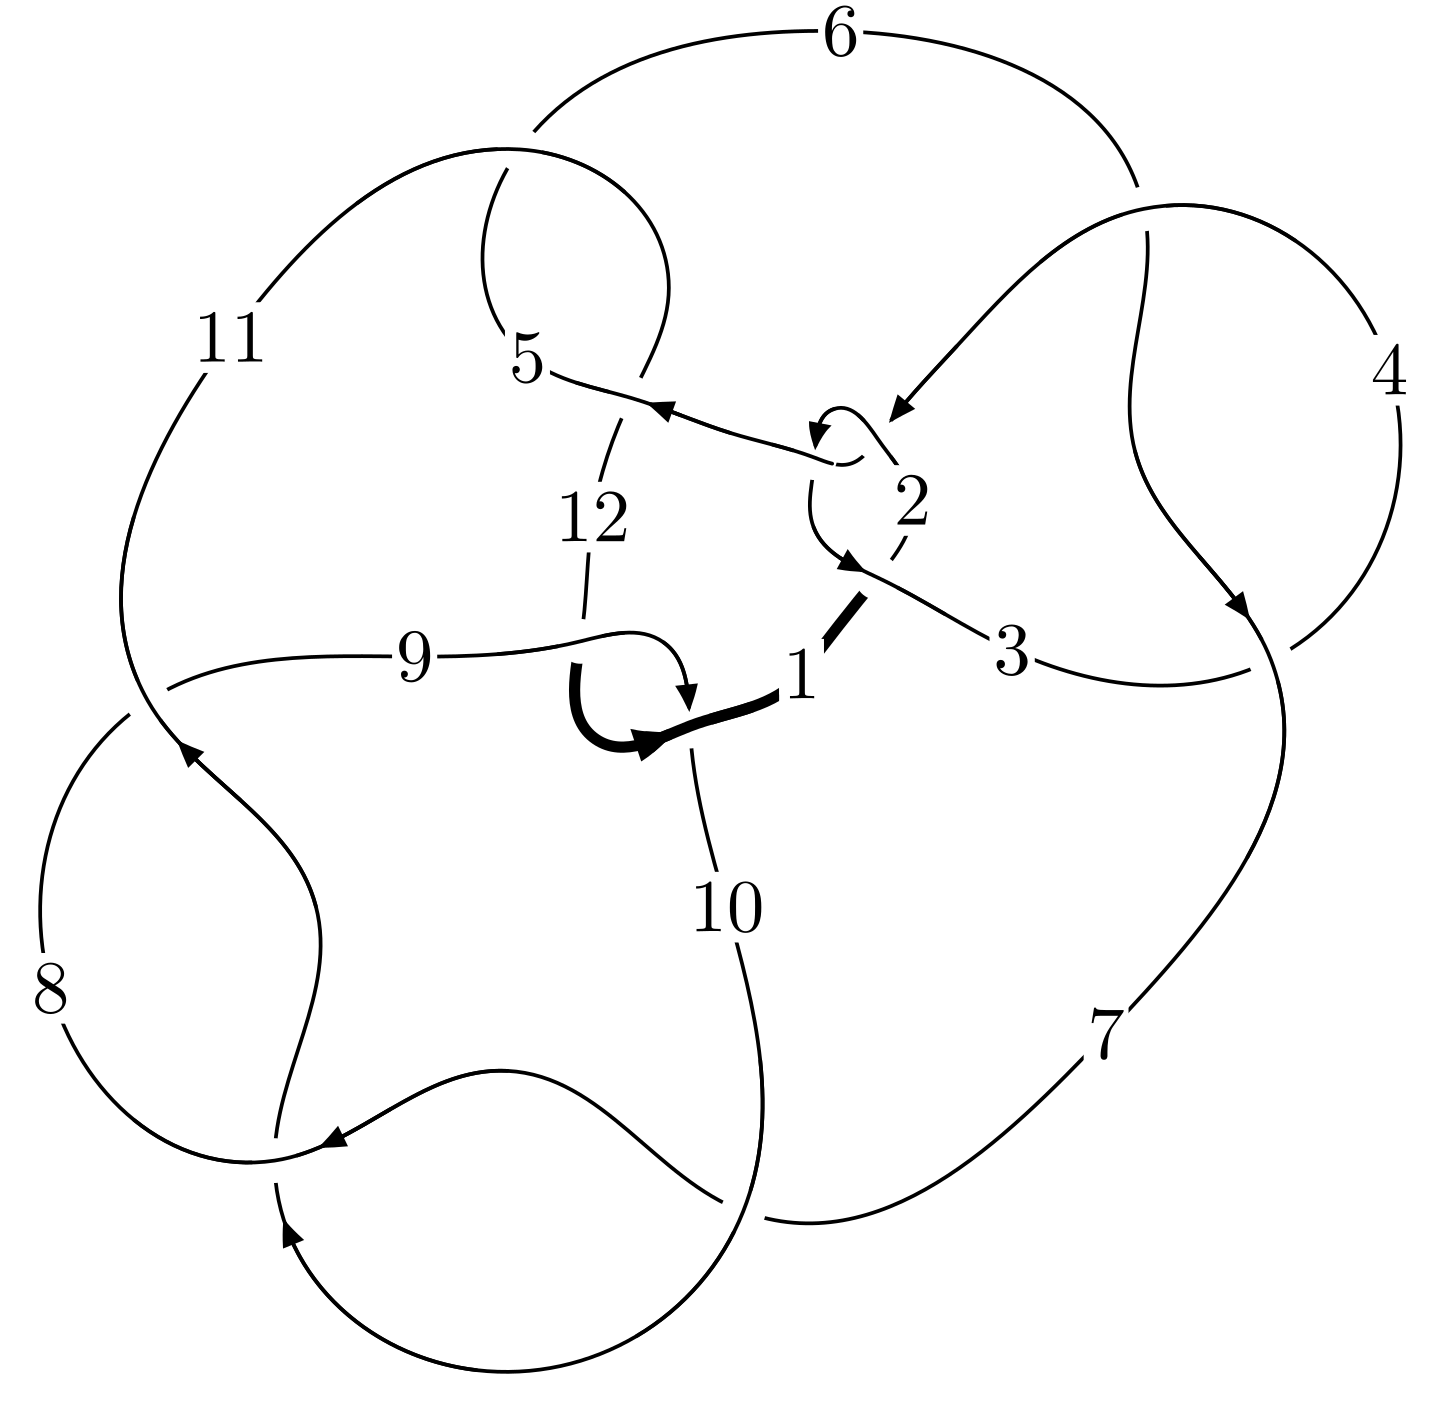
\includegraphics[width=112pt]{../../../GIT/diagram.site/Diagrams/png/2226_12n_0137.png}\\
\ \ \ A knot diagram\footnotemark}&
\allowdisplaybreaks
\textbf{Linearized knot diagam} \\
\cline{2-2}
 &
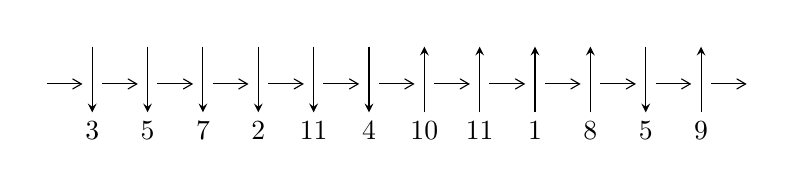
\begin{tikzpicture}[x=20pt, y=17pt]
	% nodes
	\node (C0) at (0, 0) {};
	\node (C1) at (1, 0) {};
	\node (C1U) at (1, +1) {};
	\node (C1D) at (1, -1) {3};

	\node (C2) at (2, 0) {};
	\node (C2U) at (2, +1) {};
	\node (C2D) at (2, -1) {5};

	\node (C3) at (3, 0) {};
	\node (C3U) at (3, +1) {};
	\node (C3D) at (3, -1) {7};

	\node (C4) at (4, 0) {};
	\node (C4U) at (4, +1) {};
	\node (C4D) at (4, -1) {2};

	\node (C5) at (5, 0) {};
	\node (C5U) at (5, +1) {};
	\node (C5D) at (5, -1) {11};

	\node (C6) at (6, 0) {};
	\node (C6U) at (6, +1) {};
	\node (C6D) at (6, -1) {4};

	\node (C7) at (7, 0) {};
	\node (C7U) at (7, +1) {};
	\node (C7D) at (7, -1) {10};

	\node (C8) at (8, 0) {};
	\node (C8U) at (8, +1) {};
	\node (C8D) at (8, -1) {11};

	\node (C9) at (9, 0) {};
	\node (C9U) at (9, +1) {};
	\node (C9D) at (9, -1) {1};

	\node (C10) at (10, 0) {};
	\node (C10U) at (10, +1) {};
	\node (C10D) at (10, -1) {8};

	\node (C11) at (11, 0) {};
	\node (C11U) at (11, +1) {};
	\node (C11D) at (11, -1) {5};

	\node (C12) at (12, 0) {};
	\node (C12U) at (12, +1) {};
	\node (C12D) at (12, -1) {9};
	\node (C13) at (13, 0) {};

	% arrows
	\draw[->,>={angle 60}]
	(C0) edge (C1) (C1) edge (C2) (C2) edge (C3) (C3) edge (C4) (C4) edge (C5) (C5) edge (C6) (C6) edge (C7) (C7) edge (C8) (C8) edge (C9) (C9) edge (C10) (C10) edge (C11) (C11) edge (C12) (C12) edge (C13) ;	\draw[->,>=stealth]
	(C1U) edge (C1D) (C2U) edge (C2D) (C3U) edge (C3D) (C4U) edge (C4D) (C5U) edge (C5D) (C6U) edge (C6D) (C7D) edge (C7U) (C8D) edge (C8U) (C9D) edge (C9U) (C10D) edge (C10U) (C11U) edge (C11D) (C12D) edge (C12U) ;
	\end{tikzpicture} \\
\hhline{~~} \\& 
\textbf{Solving Sequence} \\ \cline{2-2} 
 &
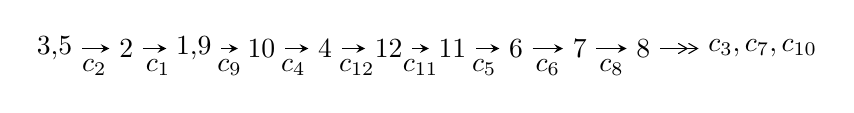
\begin{tikzpicture}[x=23pt, y=7pt]
	% node
	\node (A0) at (-1/8, 0) {3,5};
	\node (A1) at (1, 0) {2};
	\node (A2) at (33/16, 0) {1,9};
	\node (A3) at (25/8, 0) {10};
	\node (A4) at (33/8, 0) {4};
	\node (A5) at (41/8, 0) {12};
	\node (A6) at (49/8, 0) {11};
	\node (A7) at (57/8, 0) {6};
	\node (A8) at (65/8, 0) {7};
	\node (A9) at (73/8, 0) {8};
	\node (C1) at (1/2, -1) {$c_{2}$};
	\node (C2) at (3/2, -1) {$c_{1}$};
	\node (C3) at (21/8, -1) {$c_{9}$};
	\node (C4) at (29/8, -1) {$c_{4}$};
	\node (C5) at (37/8, -1) {$c_{12}$};
	\node (C6) at (45/8, -1) {$c_{11}$};
	\node (C7) at (53/8, -1) {$c_{5}$};
	\node (C8) at (61/8, -1) {$c_{6}$};
	\node (C9) at (69/8, -1) {$c_{8}$};
	\node (A10) at (11, 0) {$c_{3},c_{7},c_{10}$};

	% edge
	\draw[->,>=stealth]	
	(A0) edge (A1) (A1) edge (A2) (A2) edge (A3) (A3) edge (A4) (A4) edge (A5) (A5) edge (A6) (A6) edge (A7) (A7) edge (A8) (A8) edge (A9) ;
	\draw[->>,>={angle 60}]	
	(A9) edge (A10);
\end{tikzpicture} \\ 

\end{tabular} \\

\footnotetext{
The image of knot diagram is generated by the software ``\textbf{Draw programme}" developed by Andrew Bartholomew(\url{http://www.layer8.co.uk/maths/draw/index.htm\#Running-draw}), where we modified some parts for our purpose(\url{https://github.com/CATsTAILs/LinksPainter}).
}\phantom \\ \newline 
\centering \textbf{Ideals for irreducible components\footnotemark of $X_{\text{par}}$} 
 
\begin{align*}
I^u_{1}&=\langle 
-9.85228\times10^{76} u^{64}-6.99704\times10^{77} u^{63}+\cdots+5.10441\times10^{77} b-2.60555\times10^{76},\\
\phantom{I^u_{1}}&\phantom{= \langle  }-1.62634\times10^{77} u^{64}-1.12461\times10^{78} u^{63}+\cdots+5.10441\times10^{77} a+2.07206\times10^{79},\\
\phantom{I^u_{1}}&\phantom{= \langle  }u^{65}+7 u^{64}+\cdots-61 u+1\rangle \\
I^u_{2}&=\langle 
3 u^2 a+4 a u+u^2+b+2 a+u+1,\;- u^2 a+a^2+u^2+a- u,\;u^3+u^2-1\rangle \\
I^u_{3}&=\langle 
-4 a^2+b+a-7,\;a^3- a^2+2 a-1,\;u-1\rangle \\
I^u_{4}&=\langle 
b+u+2,\;a-2 u-3,\;u^2+u-1\rangle \\
\\
\end{align*}
\raggedright * 4 irreducible components of $\dim_{\mathbb{C}}=0$, with total 76 representations.\\
\footnotetext{All coefficients of polynomials are rational numbers. But the coefficients are sometimes approximated in decimal forms when there is not enough margin.}
\newpage
\renewcommand{\arraystretch}{1}
\centering \section*{I. $I^u_{1}= \langle -9.85\times10^{76} u^{64}-7.00\times10^{77} u^{63}+\cdots+5.10\times10^{77} b-2.61\times10^{76},\;-1.63\times10^{77} u^{64}-1.12\times10^{78} u^{63}+\cdots+5.10\times10^{77} a+2.07\times10^{79},\;u^{65}+7 u^{64}+\cdots-61 u+1 \rangle$}
\flushleft \textbf{(i) Arc colorings}\\
\begin{tabular}{m{7pt} m{180pt} m{7pt} m{180pt} }
\flushright $a_{3}=$&$\begin{pmatrix}1\\0\end{pmatrix}$ \\
\flushright $a_{5}=$&$\begin{pmatrix}0\\u\end{pmatrix}$ \\
\flushright $a_{2}=$&$\begin{pmatrix}1\\- u^2\end{pmatrix}$ \\
\flushright $a_{1}=$&$\begin{pmatrix}- u^2+1\\- u^2\end{pmatrix}$ \\
\flushright $a_{9}=$&$\begin{pmatrix}0.318614 u^{64}+2.20322 u^{63}+\cdots-187.922 u-40.5935\\0.193015 u^{64}+1.37078 u^{63}+\cdots+31.2483 u+0.0510450\end{pmatrix}$ \\
\flushright $a_{10}=$&$\begin{pmatrix}-0.181812 u^{64}-1.12398 u^{63}+\cdots-143.777 u-40.7558\\-0.312557 u^{64}-1.73228 u^{63}+\cdots+47.1225 u-0.209103\end{pmatrix}$ \\
\flushright $a_{4}=$&$\begin{pmatrix}u\\- u^3+u\end{pmatrix}$ \\
\flushright $a_{12}=$&$\begin{pmatrix}-0.0237982 u^{64}+0.139063 u^{63}+\cdots-88.0105 u-21.6619\\-1.02089 u^{64}-6.46038 u^{63}+\cdots+19.1974 u+0.00528714\end{pmatrix}$ \\
\flushright $a_{11}=$&$\begin{pmatrix}-0.0237982 u^{64}+0.139063 u^{63}+\cdots-88.0105 u-21.6619\\-0.793668 u^{64}-5.02777 u^{63}+\cdots+0.528898 u+0.310938\end{pmatrix}$ \\
\flushright $a_{6}=$&$\begin{pmatrix}-0.174107 u^{64}-1.00555 u^{63}+\cdots-15.0665 u-7.78932\\-0.246119 u^{64}-1.30818 u^{63}+\cdots+12.6788 u-0.0843556\end{pmatrix}$ \\
\flushright $a_{7}=$&$\begin{pmatrix}0.0275853 u^{64}+0.408515 u^{63}+\cdots-35.1429 u-7.46418\\0.325138 u^{64}+2.07428 u^{63}+\cdots-7.33147 u+0.243004\end{pmatrix}$ \\
\flushright $a_{8}=$&$\begin{pmatrix}0.404667 u^{64}+2.59172 u^{63}+\cdots-131.916 u-23.4724\\-0.464640 u^{64}-3.13321 u^{63}+\cdots+9.04364 u+0.172982\end{pmatrix}$\\&\end{tabular}
\flushleft \textbf{(ii) Obstruction class $= -1$}\\~\\
\flushleft \textbf{(iii) Cusp Shapes $= 1.87765 u^{64}+14.8687 u^{63}+\cdots+187.232 u+6.39873$}\\~\\
\newpage\renewcommand{\arraystretch}{1}
\flushleft \textbf{(iv) u-Polynomials at the component}\newline \\
\begin{tabular}{m{50pt}|m{274pt}}
Crossings & \hspace{64pt}u-Polynomials at each crossing \\
\hline $$\begin{aligned}c_{1}\end{aligned}$$&$\begin{aligned}
&u^{65}+35 u^{64}+\cdots+4379 u+1
\end{aligned}$\\
\hline $$\begin{aligned}c_{2},c_{4}\end{aligned}$$&$\begin{aligned}
&u^{65}-7 u^{64}+\cdots-61 u-1
\end{aligned}$\\
\hline $$\begin{aligned}c_{3},c_{6}\end{aligned}$$&$\begin{aligned}
&u^{65}-4 u^{64}+\cdots-4 u-8
\end{aligned}$\\
\hline $$\begin{aligned}c_{5},c_{11}\end{aligned}$$&$\begin{aligned}
&u^{65}-3 u^{64}+\cdots+224 u-64
\end{aligned}$\\
\hline $$\begin{aligned}c_{7},c_{8},c_{10}\end{aligned}$$&$\begin{aligned}
&u^{65}+7 u^{64}+\cdots+88 u-1
\end{aligned}$\\
\hline $$\begin{aligned}c_{9},c_{12}\end{aligned}$$&$\begin{aligned}
&u^{65}-5 u^{64}+\cdots+4 u-4
\end{aligned}$\\
\hline
\end{tabular}\\~\\
\newpage\renewcommand{\arraystretch}{1}
\flushleft \textbf{(v) Riley Polynomials at the component}\newline \\
\begin{tabular}{m{50pt}|m{274pt}}
Crossings & \hspace{64pt}Riley Polynomials at each crossing \\
\hline $$\begin{aligned}c_{1}\end{aligned}$$&$\begin{aligned}
&y^{65}-3 y^{64}+\cdots+19078099 y-1
\end{aligned}$\\
\hline $$\begin{aligned}c_{2},c_{4}\end{aligned}$$&$\begin{aligned}
&y^{65}-35 y^{64}+\cdots+4379 y-1
\end{aligned}$\\
\hline $$\begin{aligned}c_{3},c_{6}\end{aligned}$$&$\begin{aligned}
&y^{65}+24 y^{64}+\cdots+7056 y-64
\end{aligned}$\\
\hline $$\begin{aligned}c_{5},c_{11}\end{aligned}$$&$\begin{aligned}
&y^{65}-47 y^{64}+\cdots+283648 y-4096
\end{aligned}$\\
\hline $$\begin{aligned}c_{7},c_{8},c_{10}\end{aligned}$$&$\begin{aligned}
&y^{65}-55 y^{64}+\cdots+6134 y-1
\end{aligned}$\\
\hline $$\begin{aligned}c_{9},c_{12}\end{aligned}$$&$\begin{aligned}
&y^{65}-21 y^{64}+\cdots+1448 y-16
\end{aligned}$\\
\hline
\end{tabular}\\~\\
\newpage\flushleft \textbf{(vi) Complex Volumes and Cusp Shapes}
$$\begin{array}{c|c|c}  
\text{Solutions to }I^u_{1}& \I (\text{vol} + \sqrt{-1}CS) & \text{Cusp shape}\\
 \hline 
\begin{aligned}
u &= \phantom{-}0.978199 + 0.188355 I \\
a &= -0.097584 - 0.485198 I \\
b &= -0.566996 + 1.279070 I\end{aligned}
 & -1.000760 - 0.692383 I & -6.73751 + 0. I\phantom{ +0.000000I} \\ \hline\begin{aligned}
u &= \phantom{-}0.978199 - 0.188355 I \\
a &= -0.097584 + 0.485198 I \\
b &= -0.566996 - 1.279070 I\end{aligned}
 & -1.000760 + 0.692383 I & -6.73751 + 0. I\phantom{ +0.000000I} \\ \hline\begin{aligned}
u &= \phantom{-}0.989443\phantom{ +0.000000I} \\
a &= \phantom{-}0.408778\phantom{ +0.000000I} \\
b &= \phantom{-}9.34730\phantom{ +0.000000I}\end{aligned}
 & -0.561787\phantom{ +0.000000I} & -200.700\phantom{ +0.000000I} \\ \hline\begin{aligned}
u &= -0.792790 + 0.578558 I \\
a &= \phantom{-}0.102171 + 0.126924 I \\
b &= -1.09401 + 1.32036 I\end{aligned}
 & \phantom{-}11.02040 + 2.29381 I & \phantom{-0.000000 } 0 \\ \hline\begin{aligned}
u &= -0.792790 - 0.578558 I \\
a &= \phantom{-}0.102171 - 0.126924 I \\
b &= -1.09401 - 1.32036 I\end{aligned}
 & \phantom{-}11.02040 - 2.29381 I & \phantom{-0.000000 } 0 \\ \hline\begin{aligned}
u &= -0.956320 + 0.141139 I \\
a &= \phantom{-}0.48690 - 1.37332 I \\
b &= \phantom{-}0.201705 - 0.989795 I\end{aligned}
 & -4.60256 - 2.48429 I & \phantom{-}2.01382 - 9.93890 I \\ \hline\begin{aligned}
u &= -0.956320 - 0.141139 I \\
a &= \phantom{-}0.48690 + 1.37332 I \\
b &= \phantom{-}0.201705 + 0.989795 I\end{aligned}
 & -4.60256 + 2.48429 I & \phantom{-}2.01382 + 9.93890 I \\ \hline\begin{aligned}
u &= -0.683102 + 0.644381 I \\
a &= \phantom{-}1.33162 - 1.64923 I \\
b &= \phantom{-}0.818752 - 0.323057 I\end{aligned}
 & \phantom{-}4.65051 + 1.43055 I & \phantom{-}4.63524 - 5.15036 I \\ \hline\begin{aligned}
u &= -0.683102 - 0.644381 I \\
a &= \phantom{-}1.33162 + 1.64923 I \\
b &= \phantom{-}0.818752 + 0.323057 I\end{aligned}
 & \phantom{-}4.65051 - 1.43055 I & \phantom{-}4.63524 + 5.15036 I \\ \hline\begin{aligned}
u &= -0.220993 + 0.900580 I \\
a &= \phantom{-}1.71144 + 0.11133 I \\
b &= \phantom{-}0.241601 + 0.752237 I\end{aligned}
 & -0.42473 - 5.58831 I & \phantom{-0.000000 -}0. + 4.96253 I\\
 \hline 
 \end{array}$$\newpage$$\begin{array}{c|c|c}  
\text{Solutions to }I^u_{1}& \I (\text{vol} + \sqrt{-1}CS) & \text{Cusp shape}\\
 \hline 
\begin{aligned}
u &= -0.220993 - 0.900580 I \\
a &= \phantom{-}1.71144 - 0.11133 I \\
b &= \phantom{-}0.241601 - 0.752237 I\end{aligned}
 & -0.42473 + 5.58831 I & \phantom{-0.000000 } 0. - 4.96253 I \\ \hline\begin{aligned}
u &= -0.898048 + 0.623866 I \\
a &= -1.07198 + 1.80577 I \\
b &= -1.82761 + 1.02787 I\end{aligned}
 & \phantom{-}4.03132 + 3.47720 I & \phantom{-0.000000 } 0 \\ \hline\begin{aligned}
u &= -0.898048 - 0.623866 I \\
a &= -1.07198 - 1.80577 I \\
b &= -1.82761 - 1.02787 I\end{aligned}
 & \phantom{-}4.03132 - 3.47720 I & \phantom{-0.000000 } 0 \\ \hline\begin{aligned}
u &= \phantom{-}0.568826 + 0.935685 I \\
a &= -1.252080 + 0.399270 I \\
b &= -0.371291 + 1.091860 I\end{aligned}
 & \phantom{-}1.38895 + 2.95818 I & \phantom{-0.000000 } 0 \\ \hline\begin{aligned}
u &= \phantom{-}0.568826 - 0.935685 I \\
a &= -1.252080 - 0.399270 I \\
b &= -0.371291 - 1.091860 I\end{aligned}
 & \phantom{-}1.38895 - 2.95818 I & \phantom{-0.000000 } 0 \\ \hline\begin{aligned}
u &= -0.124919 + 0.887726 I \\
a &= \phantom{-}0.281399 + 0.044752 I \\
b &= -0.459233 + 0.326826 I\end{aligned}
 & \phantom{-}7.57890 - 3.09040 I & \phantom{-}6.72860 + 3.02873 I \\ \hline\begin{aligned}
u &= -0.124919 - 0.887726 I \\
a &= \phantom{-}0.281399 - 0.044752 I \\
b &= -0.459233 - 0.326826 I\end{aligned}
 & \phantom{-}7.57890 + 3.09040 I & \phantom{-}6.72860 - 3.02873 I \\ \hline\begin{aligned}
u &= -0.307741 + 1.069510 I \\
a &= -1.62825 - 0.54466 I \\
b &= -0.412336 - 1.061990 I\end{aligned}
 & \phantom{-}4.86618 - 10.28160 I & \phantom{-0.000000 } 0 \\ \hline\begin{aligned}
u &= -0.307741 - 1.069510 I \\
a &= -1.62825 + 0.54466 I \\
b &= -0.412336 + 1.061990 I\end{aligned}
 & \phantom{-}4.86618 + 10.28160 I & \phantom{-0.000000 } 0 \\ \hline\begin{aligned}
u &= -1.013850 + 0.477455 I \\
a &= -0.318794 + 0.444188 I \\
b &= \phantom{-}0.224946 - 0.486741 I\end{aligned}
 & \phantom{-}0.56978 + 4.38703 I & \phantom{-0.000000 } 0\\
 \hline 
 \end{array}$$\newpage$$\begin{array}{c|c|c}  
\text{Solutions to }I^u_{1}& \I (\text{vol} + \sqrt{-1}CS) & \text{Cusp shape}\\
 \hline 
\begin{aligned}
u &= -1.013850 - 0.477455 I \\
a &= -0.318794 - 0.444188 I \\
b &= \phantom{-}0.224946 + 0.486741 I\end{aligned}
 & \phantom{-}0.56978 - 4.38703 I & \phantom{-0.000000 } 0 \\ \hline\begin{aligned}
u &= \phantom{-}1.079610 + 0.408263 I \\
a &= \phantom{-}0.203024 + 1.130950 I \\
b &= \phantom{-}0.42767 + 1.71363 I\end{aligned}
 & -1.31032 - 2.58838 I & \phantom{-0.000000 } 0 \\ \hline\begin{aligned}
u &= \phantom{-}1.079610 - 0.408263 I \\
a &= \phantom{-}0.203024 - 1.130950 I \\
b &= \phantom{-}0.42767 - 1.71363 I\end{aligned}
 & -1.31032 + 2.58838 I & \phantom{-0.000000 } 0 \\ \hline\begin{aligned}
u &= -0.866464 + 0.780684 I \\
a &= \phantom{-}1.00474 + 1.88631 I \\
b &= -0.54581 + 2.09233 I\end{aligned}
 & \phantom{-}3.85230 + 2.93050 I & \phantom{-0.000000 } 0 \\ \hline\begin{aligned}
u &= -0.866464 - 0.780684 I \\
a &= \phantom{-}1.00474 - 1.88631 I \\
b &= -0.54581 - 2.09233 I\end{aligned}
 & \phantom{-}3.85230 - 2.93050 I & \phantom{-0.000000 } 0 \\ \hline\begin{aligned}
u &= \phantom{-}1.143920 + 0.287639 I \\
a &= \phantom{-}0.466880 + 0.894239 I \\
b &= \phantom{-}2.46022 + 2.14973 I\end{aligned}
 & -1.58736 + 0.20570 I & \phantom{-0.000000 } 0 \\ \hline\begin{aligned}
u &= \phantom{-}1.143920 - 0.287639 I \\
a &= \phantom{-}0.466880 - 0.894239 I \\
b &= \phantom{-}2.46022 - 2.14973 I\end{aligned}
 & -1.58736 - 0.20570 I & \phantom{-0.000000 } 0 \\ \hline\begin{aligned}
u &= -1.129770 + 0.340293 I \\
a &= -0.433099 + 1.075100 I \\
b &= -0.135218 + 1.075780 I\end{aligned}
 & -6.03312 + 3.48808 I & \phantom{-0.000000 } 0 \\ \hline\begin{aligned}
u &= -1.129770 - 0.340293 I \\
a &= -0.433099 - 1.075100 I \\
b &= -0.135218 - 1.075780 I\end{aligned}
 & -6.03312 - 3.48808 I & \phantom{-0.000000 } 0 \\ \hline\begin{aligned}
u &= -0.280055 + 0.763508 I \\
a &= -1.74275 + 0.40895 I \\
b &= -0.218485 + 0.488467 I\end{aligned}
 & \phantom{-}2.73256 - 3.28945 I & \phantom{-}2.80172 + 2.68321 I\\
 \hline 
 \end{array}$$\newpage$$\begin{array}{c|c|c}  
\text{Solutions to }I^u_{1}& \I (\text{vol} + \sqrt{-1}CS) & \text{Cusp shape}\\
 \hline 
\begin{aligned}
u &= -0.280055 - 0.763508 I \\
a &= -1.74275 - 0.40895 I \\
b &= -0.218485 - 0.488467 I\end{aligned}
 & \phantom{-}2.73256 + 3.28945 I & \phantom{-}2.80172 - 2.68321 I \\ \hline\begin{aligned}
u &= \phantom{-}0.802270\phantom{ +0.000000I} \\
a &= \phantom{-}0.0518504\phantom{ +0.000000I} \\
b &= -4.68222\phantom{ +0.000000I}\end{aligned}
 & \phantom{-}7.71518\phantom{ +0.000000I} & -86.2400\phantom{ +0.000000I} \\ \hline\begin{aligned}
u &= -1.100770 + 0.494345 I \\
a &= \phantom{-}0.390021 - 0.786924 I \\
b &= \phantom{-}1.74073 - 1.70018 I\end{aligned}
 & -0.66498 + 4.63908 I & \phantom{-0.000000 } 0 \\ \hline\begin{aligned}
u &= -1.100770 - 0.494345 I \\
a &= \phantom{-}0.390021 + 0.786924 I \\
b &= \phantom{-}1.74073 + 1.70018 I\end{aligned}
 & -0.66498 - 4.63908 I & \phantom{-0.000000 } 0 \\ \hline\begin{aligned}
u &= \phantom{-}1.138890 + 0.516830 I \\
a &= -0.153293 - 1.184990 I \\
b &= -1.79910 - 1.91501 I\end{aligned}
 & -4.82760 - 4.40824 I & \phantom{-0.000000 } 0 \\ \hline\begin{aligned}
u &= \phantom{-}1.138890 - 0.516830 I \\
a &= -0.153293 + 1.184990 I \\
b &= -1.79910 + 1.91501 I\end{aligned}
 & -4.82760 + 4.40824 I & \phantom{-0.000000 } 0 \\ \hline\begin{aligned}
u &= \phantom{-}0.733644 + 0.132924 I \\
a &= -2.44908 - 2.64522 I \\
b &= \phantom{-}0.25925 + 3.39498 I\end{aligned}
 & \phantom{-}0.646116 - 0.109642 I & -45.2047 + 8.8218 I \\ \hline\begin{aligned}
u &= \phantom{-}0.733644 - 0.132924 I \\
a &= -2.44908 + 2.64522 I \\
b &= \phantom{-}0.25925 - 3.39498 I\end{aligned}
 & \phantom{-}0.646116 + 0.109642 I & -45.2047 - 8.8218 I \\ \hline\begin{aligned}
u &= \phantom{-}0.212963 + 0.702410 I \\
a &= \phantom{-}1.69285 - 0.06283 I \\
b &= \phantom{-}0.285610 - 0.811517 I\end{aligned}
 & -2.18618 - 0.21906 I & -3.41412 + 0.63779 I \\ \hline\begin{aligned}
u &= \phantom{-}0.212963 - 0.702410 I \\
a &= \phantom{-}1.69285 + 0.06283 I \\
b &= \phantom{-}0.285610 + 0.811517 I\end{aligned}
 & -2.18618 + 0.21906 I & -3.41412 - 0.63779 I\\
 \hline 
 \end{array}$$\newpage$$\begin{array}{c|c|c}  
\text{Solutions to }I^u_{1}& \I (\text{vol} + \sqrt{-1}CS) & \text{Cusp shape}\\
 \hline 
\begin{aligned}
u &= -1.144350 + 0.549506 I \\
a &= \phantom{-}0.423148 - 1.005190 I \\
b &= \phantom{-}0.110767 - 1.274550 I\end{aligned}
 & \phantom{-}0.19526 + 8.22606 I & \phantom{-0.000000 } 0 \\ \hline\begin{aligned}
u &= -1.144350 - 0.549506 I \\
a &= \phantom{-}0.423148 + 1.005190 I \\
b &= \phantom{-}0.110767 + 1.274550 I\end{aligned}
 & \phantom{-}0.19526 - 8.22606 I & \phantom{-0.000000 } 0 \\ \hline\begin{aligned}
u &= \phantom{-}1.106960 + 0.690966 I \\
a &= -0.095676 + 1.306210 I \\
b &= \phantom{-}1.35935 + 1.80926 I\end{aligned}
 & -0.31021 - 8.92181 I & \phantom{-0.000000 } 0 \\ \hline\begin{aligned}
u &= \phantom{-}1.106960 - 0.690966 I \\
a &= -0.095676 - 1.306210 I \\
b &= \phantom{-}1.35935 - 1.80926 I\end{aligned}
 & -0.31021 + 8.92181 I & \phantom{-0.000000 } 0 \\ \hline\begin{aligned}
u &= -0.481434 + 0.486718 I \\
a &= \phantom{-}0.675303 - 0.696708 I \\
b &= \phantom{-}1.023720 - 0.531357 I\end{aligned}
 & \phantom{-}2.10912 - 0.34030 I & \phantom{-}3.61302 + 0.63149 I \\ \hline\begin{aligned}
u &= -0.481434 - 0.486718 I \\
a &= \phantom{-}0.675303 + 0.696708 I \\
b &= \phantom{-}1.023720 + 0.531357 I\end{aligned}
 & \phantom{-}2.10912 + 0.34030 I & \phantom{-}3.61302 - 0.63149 I \\ \hline\begin{aligned}
u &= \phantom{-}1.291860 + 0.308009 I \\
a &= -0.535246 - 0.916498 I \\
b &= -0.460659 - 1.205350 I\end{aligned}
 & -5.30684 + 1.54275 I & \phantom{-0.000000 } 0 \\ \hline\begin{aligned}
u &= \phantom{-}1.291860 - 0.308009 I \\
a &= -0.535246 + 0.916498 I \\
b &= -0.460659 + 1.205350 I\end{aligned}
 & -5.30684 - 1.54275 I & \phantom{-0.000000 } 0 \\ \hline\begin{aligned}
u &= -1.206790 + 0.570547 I \\
a &= -0.226214 + 1.184020 I \\
b &= -1.59633 + 2.09960 I\end{aligned}
 & -3.39471 + 10.94230 I & \phantom{-0.000000 } 0 \\ \hline\begin{aligned}
u &= -1.206790 - 0.570547 I \\
a &= -0.226214 - 1.184020 I \\
b &= -1.59633 - 2.09960 I\end{aligned}
 & -3.39471 - 10.94230 I & \phantom{-0.000000 } 0\\
 \hline 
 \end{array}$$\newpage$$\begin{array}{c|c|c}  
\text{Solutions to }I^u_{1}& \I (\text{vol} + \sqrt{-1}CS) & \text{Cusp shape}\\
 \hline 
\begin{aligned}
u &= \phantom{-}1.255190 + 0.475295 I \\
a &= -0.055501 - 0.186916 I \\
b &= -0.097593 - 0.921175 I\end{aligned}
 & \phantom{-}3.47356 - 1.55230 I & \phantom{-0.000000 } 0 \\ \hline\begin{aligned}
u &= \phantom{-}1.255190 - 0.475295 I \\
a &= -0.055501 + 0.186916 I \\
b &= -0.097593 + 0.921175 I\end{aligned}
 & \phantom{-}3.47356 + 1.55230 I & \phantom{-0.000000 } 0 \\ \hline\begin{aligned}
u &= \phantom{-}0.652150\phantom{ +0.000000I} \\
a &= \phantom{-}0.581302\phantom{ +0.000000I} \\
b &= -0.626898\phantom{ +0.000000I}\end{aligned}
 & -1.00335\phantom{ +0.000000I} & -10.2290\phantom{ +0.000000I} \\ \hline\begin{aligned}
u &= -1.228690 + 0.560073 I \\
a &= -0.016874 + 0.243267 I \\
b &= -0.611981 + 0.962751 I\end{aligned}
 & \phantom{-}4.31441 + 8.34885 I & \phantom{-0.000000 } 0 \\ \hline\begin{aligned}
u &= -1.228690 - 0.560073 I \\
a &= -0.016874 - 0.243267 I \\
b &= -0.611981 - 0.962751 I\end{aligned}
 & \phantom{-}4.31441 - 8.34885 I & \phantom{-0.000000 } 0 \\ \hline\begin{aligned}
u &= -0.914593 + 1.030720 I \\
a &= -0.652075 - 1.141730 I \\
b &= \phantom{-}0.23039 - 1.45733 I\end{aligned}
 & \phantom{-}9.17254 + 3.64107 I & \phantom{-0.000000 } 0 \\ \hline\begin{aligned}
u &= -0.914593 - 1.030720 I \\
a &= -0.652075 + 1.141730 I \\
b &= \phantom{-}0.23039 + 1.45733 I\end{aligned}
 & \phantom{-}9.17254 - 3.64107 I & \phantom{-0.000000 } 0 \\ \hline\begin{aligned}
u &= -0.277804 + 0.539464 I \\
a &= -1.21331 + 0.90105 I \\
b &= \phantom{-}0.374598 - 0.465447 I\end{aligned}
 & \phantom{-}1.65110 - 0.40415 I & \phantom{-}3.75505 + 0.76632 I \\ \hline\begin{aligned}
u &= -0.277804 - 0.539464 I \\
a &= -1.21331 - 0.90105 I \\
b &= \phantom{-}0.374598 + 0.465447 I\end{aligned}
 & \phantom{-}1.65110 + 0.40415 I & \phantom{-}3.75505 - 0.76632 I \\ \hline\begin{aligned}
u &= -1.250110 + 0.654083 I \\
a &= -0.032151 - 1.362680 I \\
b &= \phantom{-}1.31022 - 2.26446 I\end{aligned}
 & \phantom{-}1.9343 + 16.4466 I & \phantom{-0.000000 } 0\\
 \hline 
 \end{array}$$\newpage$$\begin{array}{c|c|c}  
\text{Solutions to }I^u_{1}& \I (\text{vol} + \sqrt{-1}CS) & \text{Cusp shape}\\
 \hline 
\begin{aligned}
u &= -1.250110 - 0.654083 I \\
a &= -0.032151 + 1.362680 I \\
b &= \phantom{-}1.31022 + 2.26446 I\end{aligned}
 & \phantom{-}1.9343 - 16.4466 I & \phantom{-0.000000 } 0 \\ \hline\begin{aligned}
u &= \phantom{-}1.46199 + 0.21591 I \\
a &= \phantom{-}0.775439 + 0.708467 I \\
b &= \phantom{-}0.671896 + 0.753763 I\end{aligned}
 & -1.34521 + 5.69764 I & \phantom{-0.000000 } 0 \\ \hline\begin{aligned}
u &= \phantom{-}1.46199 - 0.21591 I \\
a &= \phantom{-}0.775439 - 0.708467 I \\
b &= \phantom{-}0.671896 - 0.753763 I\end{aligned}
 & -1.34521 - 5.69764 I & \phantom{-0.000000 } 0 \\ \hline\begin{aligned}
u &= -1.64593\phantom{ +0.000000I} \\
a &= \phantom{-}0.300783\phantom{ +0.000000I} \\
b &= \phantom{-}0.310246\phantom{ +0.000000I}\end{aligned}
 & -7.15457\phantom{ +0.000000I} & \phantom{-0.000000 } 0 \\ \hline\begin{aligned}
u &= \phantom{-}0.0151310\phantom{ +0.000000I} \\
a &= -43.4847\phantom{ +0.000000I} \\
b &= \phantom{-}0.562042\phantom{ +0.000000I}\end{aligned}
 & \phantom{-}1.12640\phantom{ +0.000000I} & \phantom{-}9.50900\phantom{ +0.000000I}\\
 \hline 
 \end{array}$$\newpage\newpage\renewcommand{\arraystretch}{1}
\centering \section*{II. $I^u_{2}= \langle 3 u^2 a+4 a u+u^2+b+2 a+u+1,\;- u^2 a+a^2+u^2+a- u,\;u^3+u^2-1 \rangle$}
\flushleft \textbf{(i) Arc colorings}\\
\begin{tabular}{m{7pt} m{180pt} m{7pt} m{180pt} }
\flushright $a_{3}=$&$\begin{pmatrix}1\\0\end{pmatrix}$ \\
\flushright $a_{5}=$&$\begin{pmatrix}0\\u\end{pmatrix}$ \\
\flushright $a_{2}=$&$\begin{pmatrix}1\\- u^2\end{pmatrix}$ \\
\flushright $a_{1}=$&$\begin{pmatrix}- u^2+1\\- u^2\end{pmatrix}$ \\
\flushright $a_{9}=$&$\begin{pmatrix}a\\-3 u^2 a-4 a u- u^2-2 a- u-1\end{pmatrix}$ \\
\flushright $a_{10}=$&$\begin{pmatrix}u^2-1\\-2 u^2 a-3 a u-2 a- u-1\end{pmatrix}$ \\
\flushright $a_{4}=$&$\begin{pmatrix}u\\u^2+u-1\end{pmatrix}$ \\
\flushright $a_{12}=$&$\begin{pmatrix}0\\2 u^2 a+3 a u+2 u^2+2 a+2 u+2\end{pmatrix}$ \\
\flushright $a_{11}=$&$\begin{pmatrix}0\\2 u^2 a+3 a u+2 u^2+2 a+2 u+2\end{pmatrix}$ \\
\flushright $a_{6}=$&$\begin{pmatrix}0\\u\end{pmatrix}$ \\
\flushright $a_{7}=$&$\begin{pmatrix}u^2-1\\u^2\end{pmatrix}$ \\
\flushright $a_{8}=$&$\begin{pmatrix}a\\u^2 a+2 a u+2 u^2+2 a+2 u+2\end{pmatrix}$\\&\end{tabular}
\flushleft \textbf{(ii) Obstruction class $= 1$}\\~\\
\flushleft \textbf{(iii) Cusp Shapes $= 21 u^2 a+39 a u+11 u^2+24 a+19 u+26$}\\~\\
\newpage\renewcommand{\arraystretch}{1}
\flushleft \textbf{(iv) u-Polynomials at the component}\newline \\
\begin{tabular}{m{50pt}|m{274pt}}
Crossings & \hspace{64pt}u-Polynomials at each crossing \\
\hline $$\begin{aligned}c_{1},c_{3}\end{aligned}$$&$\begin{aligned}
&(u^3- u^2+2 u-1)^2
\end{aligned}$\\
\hline $$\begin{aligned}c_{2}\end{aligned}$$&$\begin{aligned}
&(u^3+u^2-1)^2
\end{aligned}$\\
\hline $$\begin{aligned}c_{4}\end{aligned}$$&$\begin{aligned}
&(u^3- u^2+1)^2
\end{aligned}$\\
\hline $$\begin{aligned}c_{5},c_{11}\end{aligned}$$&$\begin{aligned}
&u^6
\end{aligned}$\\
\hline $$\begin{aligned}c_{6}\end{aligned}$$&$\begin{aligned}
&(u^3+u^2+2 u+1)^2
\end{aligned}$\\
\hline $$\begin{aligned}c_{7},c_{8},c_{9}\end{aligned}$$&$\begin{aligned}
&(u^2- u-1)^3
\end{aligned}$\\
\hline $$\begin{aligned}c_{10},c_{12}\end{aligned}$$&$\begin{aligned}
&(u^2+u-1)^3
\end{aligned}$\\
\hline
\end{tabular}\\~\\
\newpage\renewcommand{\arraystretch}{1}
\flushleft \textbf{(v) Riley Polynomials at the component}\newline \\
\begin{tabular}{m{50pt}|m{274pt}}
Crossings & \hspace{64pt}Riley Polynomials at each crossing \\
\hline $$\begin{aligned}c_{1},c_{3},c_{6}\end{aligned}$$&$\begin{aligned}
&(y^3+3 y^2+2 y-1)^2
\end{aligned}$\\
\hline $$\begin{aligned}c_{2},c_{4}\end{aligned}$$&$\begin{aligned}
&(y^3- y^2+2 y-1)^2
\end{aligned}$\\
\hline $$\begin{aligned}c_{5},c_{11}\end{aligned}$$&$\begin{aligned}
&y^6
\end{aligned}$\\
\hline $$\begin{aligned}c_{7},c_{8},c_{9}\\c_{10},c_{12}\end{aligned}$$&$\begin{aligned}
&(y^2-3 y+1)^3
\end{aligned}$\\
\hline
\end{tabular}\\~\\
\newpage\flushleft \textbf{(vi) Complex Volumes and Cusp Shapes}
$$\begin{array}{c|c|c}  
\text{Solutions to }I^u_{2}& \I (\text{vol} + \sqrt{-1}CS) & \text{Cusp shape}\\
 \hline 
\begin{aligned}
u &= -0.877439 + 0.744862 I \\
a &= \phantom{-}0.485107 + 0.807858 I \\
b &= -0.67924 + 1.71765 I\end{aligned}
 & \phantom{-}11.90680 + 2.82812 I & \phantom{-}7.63548 - 4.05775 I \\ \hline\begin{aligned}
u &= -0.877439 + 0.744862 I \\
a &= -1.27003 - 2.11500 I \\
b &= \phantom{-}0.55668 - 2.46251 I\end{aligned}
 & \phantom{-}4.01109 + 2.82812 I & \phantom{-}22.3213 + 9.8050 I \\ \hline\begin{aligned}
u &= -0.877439 - 0.744862 I \\
a &= \phantom{-}0.485107 - 0.807858 I \\
b &= -0.67924 - 1.71765 I\end{aligned}
 & \phantom{-}11.90680 - 2.82812 I & \phantom{-}7.63548 + 4.05775 I \\ \hline\begin{aligned}
u &= -0.877439 - 0.744862 I \\
a &= -1.27003 + 2.11500 I \\
b &= \phantom{-}0.55668 + 2.46251 I\end{aligned}
 & \phantom{-}4.01109 - 2.82812 I & \phantom{-}22.3213 - 9.8050 I \\ \hline\begin{aligned}
u &= \phantom{-}0.754878\phantom{ +0.000000I} \\
a &= -0.696013\phantom{ +0.000000I} \\
b &= \phantom{-}2.35878\phantom{ +0.000000I}\end{aligned}
 & -0.126494\phantom{ +0.000000I} & \phantom{-}1.08690\phantom{ +0.000000I} \\ \hline\begin{aligned}
u &= \phantom{-}0.754878\phantom{ +0.000000I} \\
a &= \phantom{-}0.265853\phantom{ +0.000000I} \\
b &= -4.11365\phantom{ +0.000000I}\end{aligned}
 & \phantom{-}7.76919\phantom{ +0.000000I} & \phantom{-}64.0000\phantom{ +0.000000I}\\
 \hline 
 \end{array}$$\newpage\newpage\renewcommand{\arraystretch}{1}
\centering \section*{III. $I^u_{3}= \langle -4 a^2+b+a-7,\;a^3- a^2+2 a-1,\;u-1 \rangle$}
\flushleft \textbf{(i) Arc colorings}\\
\begin{tabular}{m{7pt} m{180pt} m{7pt} m{180pt} }
\flushright $a_{3}=$&$\begin{pmatrix}1\\0\end{pmatrix}$ \\
\flushright $a_{5}=$&$\begin{pmatrix}0\\1\end{pmatrix}$ \\
\flushright $a_{2}=$&$\begin{pmatrix}1\\-1\end{pmatrix}$ \\
\flushright $a_{1}=$&$\begin{pmatrix}0\\-1\end{pmatrix}$ \\
\flushright $a_{9}=$&$\begin{pmatrix}a\\4 a^2- a+7\end{pmatrix}$ \\
\flushright $a_{10}=$&$\begin{pmatrix}a\\4 a^2-2 a+7\end{pmatrix}$ \\
\flushright $a_{4}=$&$\begin{pmatrix}1\\0\end{pmatrix}$ \\
\flushright $a_{12}=$&$\begin{pmatrix}a^2\\3 a^2- a+3\end{pmatrix}$ \\
\flushright $a_{11}=$&$\begin{pmatrix}a^2\\2 a^2- a+3\end{pmatrix}$ \\
\flushright $a_{6}=$&$\begin{pmatrix}a^2+a-1\\0\end{pmatrix}$ \\
\flushright $a_{7}=$&$\begin{pmatrix}a^2+a-1\\0\end{pmatrix}$ \\
\flushright $a_{8}=$&$\begin{pmatrix}a^2\\3 a^2- a+5\end{pmatrix}$\\&\end{tabular}
\flushleft \textbf{(ii) Obstruction class $= 1$}\\~\\
\flushleft \textbf{(iii) Cusp Shapes $= 53 a^2-32 a+92$}\\~\\
\newpage\renewcommand{\arraystretch}{1}
\flushleft \textbf{(iv) u-Polynomials at the component}\newline \\
\begin{tabular}{m{50pt}|m{274pt}}
Crossings & \hspace{64pt}u-Polynomials at each crossing \\
\hline $$\begin{aligned}c_{1},c_{2}\end{aligned}$$&$\begin{aligned}
&(u-1)^3
\end{aligned}$\\
\hline $$\begin{aligned}c_{3},c_{6}\end{aligned}$$&$\begin{aligned}
&u^3
\end{aligned}$\\
\hline $$\begin{aligned}c_{4}\end{aligned}$$&$\begin{aligned}
&(u+1)^3
\end{aligned}$\\
\hline $$\begin{aligned}c_{5}\end{aligned}$$&$\begin{aligned}
&u^3-3 u^2+2 u+1
\end{aligned}$\\
\hline $$\begin{aligned}c_{7},c_{8}\end{aligned}$$&$\begin{aligned}
&u^3- u^2+1
\end{aligned}$\\
\hline $$\begin{aligned}c_{9}\end{aligned}$$&$\begin{aligned}
&u^3+u^2+2 u+1
\end{aligned}$\\
\hline $$\begin{aligned}c_{10}\end{aligned}$$&$\begin{aligned}
&u^3+u^2-1
\end{aligned}$\\
\hline $$\begin{aligned}c_{11}\end{aligned}$$&$\begin{aligned}
&u^3+3 u^2+2 u-1
\end{aligned}$\\
\hline $$\begin{aligned}c_{12}\end{aligned}$$&$\begin{aligned}
&u^3- u^2+2 u-1
\end{aligned}$\\
\hline
\end{tabular}\\~\\
\newpage\renewcommand{\arraystretch}{1}
\flushleft \textbf{(v) Riley Polynomials at the component}\newline \\
\begin{tabular}{m{50pt}|m{274pt}}
Crossings & \hspace{64pt}Riley Polynomials at each crossing \\
\hline $$\begin{aligned}c_{1},c_{2},c_{4}\end{aligned}$$&$\begin{aligned}
&(y-1)^3
\end{aligned}$\\
\hline $$\begin{aligned}c_{3},c_{6}\end{aligned}$$&$\begin{aligned}
&y^3
\end{aligned}$\\
\hline $$\begin{aligned}c_{5},c_{11}\end{aligned}$$&$\begin{aligned}
&y^3-5 y^2+10 y-1
\end{aligned}$\\
\hline $$\begin{aligned}c_{7},c_{8},c_{10}\end{aligned}$$&$\begin{aligned}
&y^3- y^2+2 y-1
\end{aligned}$\\
\hline $$\begin{aligned}c_{9},c_{12}\end{aligned}$$&$\begin{aligned}
&y^3+3 y^2+2 y-1
\end{aligned}$\\
\hline
\end{tabular}\\~\\
\newpage\flushleft \textbf{(vi) Complex Volumes and Cusp Shapes}
$$\begin{array}{c|c|c}  
\text{Solutions to }I^u_{3}& \I (\text{vol} + \sqrt{-1}CS) & \text{Cusp shape}\\
 \hline 
\begin{aligned}
u &= \phantom{-}1.00000\phantom{ +0.000000I} \\
a &= \phantom{-}0.215080 + 1.307140 I \\
b &= \phantom{-}0.135484 + 0.941977 I\end{aligned}
 & -4.66906 + 2.82812 I & -2.98758 - 12.02771 I \\ \hline\begin{aligned}
u &= \phantom{-}1.00000\phantom{ +0.000000I} \\
a &= \phantom{-}0.215080 - 1.307140 I \\
b &= \phantom{-}0.135484 - 0.941977 I\end{aligned}
 & -4.66906 - 2.82812 I & -2.98758 + 12.02771 I \\ \hline\begin{aligned}
u &= \phantom{-}1.00000\phantom{ +0.000000I} \\
a &= \phantom{-}0.569840\phantom{ +0.000000I} \\
b &= \phantom{-}7.72903\phantom{ +0.000000I}\end{aligned}
 & -0.531480\phantom{ +0.000000I} & \phantom{-}90.9750\phantom{ +0.000000I}\\
 \hline 
 \end{array}$$\newpage\newpage\renewcommand{\arraystretch}{1}
\centering \section*{IV. $I^u_{4}= \langle b+u+2,\;a-2 u-3,\;u^2+u-1 \rangle$}
\flushleft \textbf{(i) Arc colorings}\\
\begin{tabular}{m{7pt} m{180pt} m{7pt} m{180pt} }
\flushright $a_{3}=$&$\begin{pmatrix}1\\0\end{pmatrix}$ \\
\flushright $a_{5}=$&$\begin{pmatrix}0\\u\end{pmatrix}$ \\
\flushright $a_{2}=$&$\begin{pmatrix}1\\u-1\end{pmatrix}$ \\
\flushright $a_{1}=$&$\begin{pmatrix}u\\u-1\end{pmatrix}$ \\
\flushright $a_{9}=$&$\begin{pmatrix}2 u+3\\- u-2\end{pmatrix}$ \\
\flushright $a_{10}=$&$\begin{pmatrix}2 u+3\\- u-2\end{pmatrix}$ \\
\flushright $a_{4}=$&$\begin{pmatrix}u\\- u+1\end{pmatrix}$ \\
\flushright $a_{12}=$&$\begin{pmatrix}u\\u-1\end{pmatrix}$ \\
\flushright $a_{11}=$&$\begin{pmatrix}u\\- u\end{pmatrix}$ \\
\flushright $a_{6}=$&$\begin{pmatrix}-2 u+1\\3 u-1\end{pmatrix}$ \\
\flushright $a_{7}=$&$\begin{pmatrix}- u\\u\end{pmatrix}$ \\
\flushright $a_{8}=$&$\begin{pmatrix}u+3\\-2\end{pmatrix}$\\&\end{tabular}
\flushleft \textbf{(ii) Obstruction class $= 1$}\\~\\
\flushleft \textbf{(iii) Cusp Shapes $= -49$}\\~\\
\newpage\renewcommand{\arraystretch}{1}
\flushleft \textbf{(iv) u-Polynomials at the component}\newline \\
\begin{tabular}{m{50pt}|m{274pt}}
Crossings & \hspace{64pt}u-Polynomials at each crossing \\
\hline $$\begin{aligned}c_{1},c_{11}\end{aligned}$$&$\begin{aligned}
&u^2-3 u+1
\end{aligned}$\\
\hline $$\begin{aligned}c_{2},c_{3}\end{aligned}$$&$\begin{aligned}
&u^2+u-1
\end{aligned}$\\
\hline $$\begin{aligned}c_{4},c_{6}\end{aligned}$$&$\begin{aligned}
&u^2- u-1
\end{aligned}$\\
\hline $$\begin{aligned}c_{5}\end{aligned}$$&$\begin{aligned}
&u^2+3 u+1
\end{aligned}$\\
\hline $$\begin{aligned}c_{7},c_{8}\end{aligned}$$&$\begin{aligned}
&(u+1)^2
\end{aligned}$\\
\hline $$\begin{aligned}c_{9},c_{12}\end{aligned}$$&$\begin{aligned}
&u^2
\end{aligned}$\\
\hline $$\begin{aligned}c_{10}\end{aligned}$$&$\begin{aligned}
&(u-1)^2
\end{aligned}$\\
\hline
\end{tabular}\\~\\
\newpage\renewcommand{\arraystretch}{1}
\flushleft \textbf{(v) Riley Polynomials at the component}\newline \\
\begin{tabular}{m{50pt}|m{274pt}}
Crossings & \hspace{64pt}Riley Polynomials at each crossing \\
\hline $$\begin{aligned}c_{1},c_{5},c_{11}\end{aligned}$$&$\begin{aligned}
&y^2-7 y+1
\end{aligned}$\\
\hline $$\begin{aligned}c_{2},c_{3},c_{4}\\c_{6}\end{aligned}$$&$\begin{aligned}
&y^2-3 y+1
\end{aligned}$\\
\hline $$\begin{aligned}c_{7},c_{8},c_{10}\end{aligned}$$&$\begin{aligned}
&(y-1)^2
\end{aligned}$\\
\hline $$\begin{aligned}c_{9},c_{12}\end{aligned}$$&$\begin{aligned}
&y^2
\end{aligned}$\\
\hline
\end{tabular}\\~\\
\newpage\flushleft \textbf{(vi) Complex Volumes and Cusp Shapes}
$$\begin{array}{c|c|c}  
\text{Solutions to }I^u_{4}& \I (\text{vol} + \sqrt{-1}CS) & \text{Cusp shape}\\
 \hline 
\begin{aligned}
u &= \phantom{-}0.618034\phantom{ +0.000000I} \\
a &= \phantom{-}4.23607\phantom{ +0.000000I} \\
b &= -2.61803\phantom{ +0.000000I}\end{aligned}
 & \phantom{-}0.657974\phantom{ +0.000000I} & -49.0000\phantom{ +0.000000I} \\ \hline\begin{aligned}
u &= -1.61803\phantom{ +0.000000I} \\
a &= -0.236068\phantom{ +0.000000I} \\
b &= -0.381966\phantom{ +0.000000I}\end{aligned}
 & -7.23771\phantom{ +0.000000I} & -49.0000\phantom{ +0.000000I}\\
 \hline 
 \end{array}$$\newpage
\newpage\renewcommand{\arraystretch}{1}
\centering \section*{ V. u-Polynomials}
\begin{tabular}{m{50pt}|m{274pt}}
Crossings & \hspace{64pt}u-Polynomials at each crossing \\
\hline $$\begin{aligned}c_{1}\end{aligned}$$&$\begin{aligned}
&(u-1)^3(u^2-3 u+1)(u^3- u^2+2 u-1)^2\\
&\cdot(u^{65}+35 u^{64}+\cdots+4379 u+1)
\end{aligned}$\\
\hline $$\begin{aligned}c_{2}\end{aligned}$$&$\begin{aligned}
&((u-1)^3)(u^2+u-1)(u^3+u^2-1)^2(u^{65}-7 u^{64}+\cdots-61 u-1)
\end{aligned}$\\
\hline $$\begin{aligned}c_{3}\end{aligned}$$&$\begin{aligned}
&u^3(u^2+u-1)(u^3- u^2+2 u-1)^{2}(u^{65}-4 u^{64}+\cdots-4 u-8)
\end{aligned}$\\
\hline $$\begin{aligned}c_{4}\end{aligned}$$&$\begin{aligned}
&((u+1)^3)(u^2- u-1)(u^3- u^2+1)^2(u^{65}-7 u^{64}+\cdots-61 u-1)
\end{aligned}$\\
\hline $$\begin{aligned}c_{5}\end{aligned}$$&$\begin{aligned}
&u^6(u^2+3 u+1)(u^{3}-3 u^{2}+2 u+1)(u^{65}-3 u^{64}+\cdots+224 u-64)
\end{aligned}$\\
\hline $$\begin{aligned}c_{6}\end{aligned}$$&$\begin{aligned}
&u^3(u^2- u-1)(u^3+u^2+2 u+1)^{2}(u^{65}-4 u^{64}+\cdots-4 u-8)
\end{aligned}$\\
\hline $$\begin{aligned}c_{7},c_{8}\end{aligned}$$&$\begin{aligned}
&((u+1)^2)(u^2- u-1)^3(u^3- u^2+1)(u^{65}+7 u^{64}+\cdots+88 u-1)
\end{aligned}$\\
\hline $$\begin{aligned}c_{9}\end{aligned}$$&$\begin{aligned}
&u^2(u^2- u-1)^3(u^3+u^2+2 u+1)(u^{65}-5 u^{64}+\cdots+4 u-4)
\end{aligned}$\\
\hline $$\begin{aligned}c_{10}\end{aligned}$$&$\begin{aligned}
&((u-1)^2)(u^2+u-1)^3(u^3+u^2-1)(u^{65}+7 u^{64}+\cdots+88 u-1)
\end{aligned}$\\
\hline $$\begin{aligned}c_{11}\end{aligned}$$&$\begin{aligned}
&u^6(u^2-3 u+1)(u^{3}+3 u^{2}+2 u-1)(u^{65}-3 u^{64}+\cdots+224 u-64)
\end{aligned}$\\
\hline $$\begin{aligned}c_{12}\end{aligned}$$&$\begin{aligned}
&u^2(u^2+u-1)^3(u^3- u^2+2 u-1)(u^{65}-5 u^{64}+\cdots+4 u-4)
\end{aligned}$\\
\hline
\end{tabular}\newpage\renewcommand{\arraystretch}{1}
\centering \section*{ VI. Riley Polynomials}
\begin{tabular}{m{50pt}|m{274pt}}
Crossings & \hspace{64pt}Riley Polynomials at each crossing \\
\hline $$\begin{aligned}c_{1}\end{aligned}$$&$\begin{aligned}
&(y-1)^3(y^2-7 y+1)(y^3+3 y^2+2 y-1)^2\\
&\cdot(y^{65}-3 y^{64}+\cdots+19078099 y-1)
\end{aligned}$\\
\hline $$\begin{aligned}c_{2},c_{4}\end{aligned}$$&$\begin{aligned}
&(y-1)^3(y^2-3 y+1)(y^3- y^2+2 y-1)^2\\
&\cdot(y^{65}-35 y^{64}+\cdots+4379 y-1)
\end{aligned}$\\
\hline $$\begin{aligned}c_{3},c_{6}\end{aligned}$$&$\begin{aligned}
&y^3(y^2-3 y+1)(y^{3}+3 y^{2}+2 y-1)^{2}(y^{65}+24 y^{64}+\cdots+7056 y-64)
\end{aligned}$\\
\hline $$\begin{aligned}c_{5},c_{11}\end{aligned}$$&$\begin{aligned}
&y^6(y^2-7 y+1)(y^3-5 y^2+10 y-1)\\
&\cdot(y^{65}-47 y^{64}+\cdots+283648 y-4096)
\end{aligned}$\\
\hline $$\begin{aligned}c_{7},c_{8},c_{10}\end{aligned}$$&$\begin{aligned}
&(y-1)^2(y^2-3 y+1)^3(y^3- y^2+2 y-1)\\
&\cdot(y^{65}-55 y^{64}+\cdots+6134 y-1)
\end{aligned}$\\
\hline $$\begin{aligned}c_{9},c_{12}\end{aligned}$$&$\begin{aligned}
&y^2(y^2-3 y+1)^3(y^{3}+3 y^{2}+2 y-1)(y^{65}-21 y^{64}+\cdots+1448 y-16)
\end{aligned}$\\
\hline
\end{tabular}
\vskip 2pc
\end{document}